\documentclass[a4paper]{article}

  \usepackage{fullpage} % Package to use full page
  \usepackage{parskip} % Package to tweak paragraph skipping
  \usepackage{tikz} % Package for drawing
  \usepackage{amsmath}
  \usepackage{siunitx} % Package for scientific units
  \usepackage{amsfonts}
  \usepackage{amssymb}
  \usepackage{hyperref}
  \usepackage[utf8]{inputenc}
  \usepackage[english]{babel}
  \usepackage{multicol}
  \usepackage{graphicx} % Package for including images
  \graphicspath{ {./images/} }
  
  \newcommand\tab[1][0.5cm]{\hspace*{#1}}
  
  \title{Lab 7}
  \author{Adrian Darian}
  \date{10/26/2020}
  
  \begin{document}
  
\maketitle
  
\section*{Discussion Section 2}

\section*{Assignment:}
\begin{itemize}
    \item[1.] Use Monte Carlo Integration to integrate: \\
    \tab $f(x) = \sqrt{1 + \frac{1}{2x}}$ from 1 to 3 \\
    \tab Note: For this example skip the by hand integration and simply supply the plots. \\
    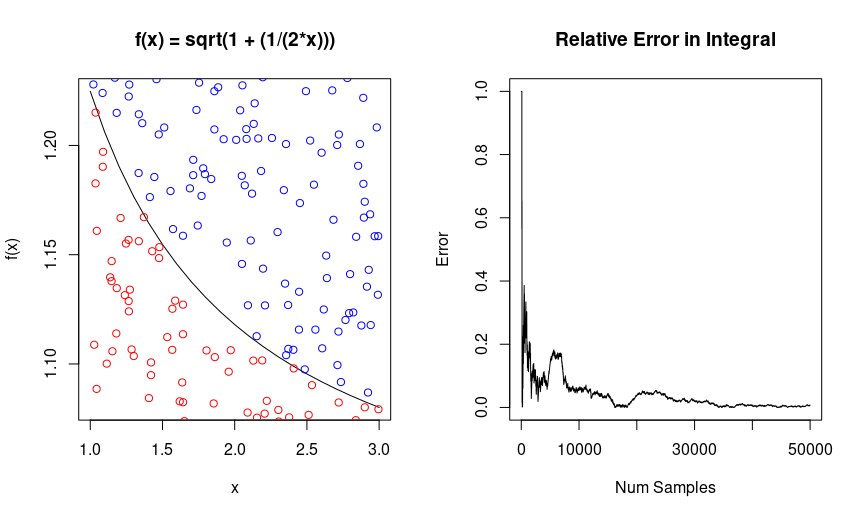
\includegraphics[scale=0.5]{Rplot.png}
    \item[2.] Provide both a write-up of your solution by hand (1 Point), and figures from
    your Monte Carlo Integration (2 Points) of \\
    \tab $\int _1^5\frac{1}{x^2\left(x^2+25\right)}dx$ \\
    \begin{itemize}
      \item 
    \end{itemize}
    \item[3.] Another function of your choosing from the list below. But you must show
    both your by hand integration and your results from Monte Carlo Integration.
    \tab Integrate f(x) = x −1/3 + x/10 from 0 to 1.
\end{itemize}

  
\end{document}